%%%%%%%%%%%%%%%%%%%%%%%%%%%%%%%%%%%%%%%%%
% Short Sectioned Assignment LaTeX Template Version 1.0 (5/5/12)
% This template has been downloaded from: http://www.LaTeXTemplates.com
% Original author:  Frits Wenneker (http://www.howtotex.com)
% License: CC BY-NC-SA 3.0 (http://creativecommons.org/licenses/by-nc-sa/3.0/)
%%%%%%%%%%%%%%%%%%%%%%%%%%%%%%%%%%%%%%%%%

%----------------------------------------------------------------------------------------
%	PACKAGES AND OTHER DOCUMENT CONFIGURATIONS
%----------------------------------------------------------------------------------------

\documentclass[paper=a4, fontsize=11pt]{scrartcl} % A4 paper and 11pt font size

% ---- Entrada y salida de texto -----

\usepackage[T1]{fontenc} % Use 8-bit encoding that has 256 glyphs
\usepackage[utf8]{inputenc}
%\usepackage{fourier} % Use the Adobe Utopia font for the document - comment this line to return to the LaTeX default


\usepackage[utf8]{inputenc}
\usepackage[T1]{fontenc}
\usepackage[spanish]{babel}
\usepackage{times}

\usepackage{color}
\definecolor{gray97}{gray}{.97}
\definecolor{gray75}{gray}{.75}
\definecolor{gray45}{gray}{.45}

\usepackage{listings}
\lstset{ frame=Ltb,
	framerule=0pt,
	aboveskip=0.5cm,
	framextopmargin=3pt,
	framexbottommargin=3pt,
	framexleftmargin=0.4cm,
	framesep=0pt,
	rulesep=.4pt,
	backgroundcolor=\color{gray97},
	rulesepcolor=\color{black},
	%
	stringstyle=\ttfamily,
	showstringspaces = false,
	basicstyle=\small\ttfamily,
	commentstyle=\color{gray45},
	keywordstyle=\bfseries,
	%
	numbers=left,
	numbersep=15pt,
	numberstyle=\tiny,
	numberfirstline = false,
	breaklines=true,
}

% minimizar fragmentado de listados
\lstnewenvironment{listing}[1][]
{\lstset{#1}\pagebreak[0]}{\pagebreak[0]}

\lstdefinestyle{consola}
{basicstyle=\scriptsize\bf\ttfamily,
	backgroundcolor=\color{gray75},
}

\lstdefinestyle{C}
{language=C,
}
% ---- Idioma --------

\usepackage[spanish, es-tabla]{babel} % Selecciona el español para palabras introducidas automáticamente, p.ej. "septiembre" en la fecha y especifica que se use la palabra Tabla en vez de Cuadro
% ---- Otros paquetes ----

\usepackage{amsmath,amsfonts,amsthm} % Math packages
%\usepackage{graphics,graphicx, floatrow} %para incluir imágenes y notas en las imágenes
\usepackage{graphics,graphicx, float} %para incluir imágenes y colocarlas

% Para hacer tablas comlejas
%\usepackage{multirow}
%\usepackage{threeparttable}

%\usepackage{sectsty} % Allows customizing section commands
%\allsectionsfont{\centering \normalfont\scshape} % Make all sections centered, the default font and small caps

\usepackage{fancyhdr} % Custom headers and footers
\pagestyle{fancyplain} % Makes all pages in the document conform to the custom headers and footers
\fancyhead{} % No page header - if you want one, create it in the same way as the footers below
\fancyfoot[L]{} % Empty left footer
\fancyfoot[C]{} % Empty center footer
\fancyfoot[R]{\thepage} % Page numbering for right footer
\renewcommand{\headrulewidth}{0pt} % Remove header underlines
\renewcommand{\footrulewidth}{0pt} % Remove footer underlines
\setlength{\headheight}{13.6pt} % Customize the height of the header

\numberwithin{equation}{section} % Number equations within sections (i.e. 1.1, 1.2, 2.1, 2.2 instead of 1, 2, 3, 4)
\numberwithin{figure}{section} % Number figures within sections (i.e. 1.1, 1.2, 2.1, 2.2 instead of 1, 2, 3, 4)
\numberwithin{table}{section} % Number tables within sections (i.e. 1.1, 1.2, 2.1, 2.2 instead of 1, 2, 3, 4)

\setlength\parindent{0pt} % Removes all indentation from paragraphs - comment this line for an assignment with lots of text

\newcommand{\horrule}[1]{\rule{\linewidth}{#1}} % Create horizontal rule command with 1 argument of height


\begin{document}
\title{
\normalfont \normalsize 
\textsc{{\bf Metaheurísticas (2015-16) \\ Grado en Ingeniería Informática \\ Universidad de Granada} \\ [25pt] % Your university, school and/or department name(s)
\horrule{0.5pt} \\[0.4cm] % Thin top horizontal rule
\huge Práctica 2: Búsqueda por trayectorias múltiples para el problema de la Selección de características \\ % The assignment title
\horrule{2pt} \\[0.5cm] % Thick bottom horizontal rule
}}
\author{Miguel López Campos\\ 54120359W\\ miguelberja@correo.ugr.es\\ Grupo Viernes 18:30} % Nombre y apellidos


\date{\normalsize\today} % Incluye la fecha actual
%----------------------------------------------------------------------------------------
% DOCUMENTO
%----------------------------------------------------------------------------------------


	
	\maketitle % Muestra el Título
	\newpage %inserta un salto de página
	
	\tableofcontents % para generar el índice de contenidos
	\listoffigures

	
	\newpage
	
	\
	
	
	
	\section{Descripción del problema}
	El problema que estamos abordando es la selección de características. Este problema es muy útil en el campo de "machine learning".
	\\
	\\
	Tenemos un conjunto de datos de entrenamiento y otro de validación, ambos etiquetados o clasificados. Lo que queremos hacer es 'aprender' una función que a partir de las características del conjunto de datos de entrenamiento, nos permita estimar el etiquetado de otros vectores de características. Lo que nosotros queremos hacer es eliminar las características que no son relevantes en el problema, eliminando de esta manera ruido en el conjunto de datos y mejorando la eficiencia de nuestro clasificador. Es decir, no sólo mejoraremos el tiempo, si no muy probablemente la calidad de nuestras soluciones también (en cuanto al error se refiere).
	\\
	\\
	La gran dificultad de este problema radica en el gran número de soluciones posibles, llevándonos al punto de que un algoritmo Greedy que nos garantice la solución óptima podría llevarnos días de ejecución para determinados problemas. Es por esto por lo que tenemos que usar Metaheurísticas. Necesitamos soluciones buenas (aunque no sea la mejor) en un tiempo menor.
	\\
	\\
	Nosotros usaremos para clasificar el algoritmo 3NN. Lo que hace este algoritmo es calcular la distancia euclídea entre el vector de características al cual queremos estimar una clase y el resto de vectores de características del conjunto de entrenamiento. Lo que hace el 3NN es coger los 3 elementos menos distantes y la clase mayoritaria entre esos 3 será la estimación que haremos.
	\\
	\\
	Validaremos con la técnica 5x2 Cross Validation. Usaremos 5 particiones de los datos distintas al 50\% (y aleatorias) y aprenderemos el clasificador con una submuestra y validaremos con la otra y después al contrario. Con esta técnica tendremos el porcentaje de acierto, que nos servirá para ver la calidad de nuestro algoritmo.
	\\
	\\
	Otros datos con los que valoraremos la calidad de nuestros algoritmos serán los tiempos de ejeución y los porcentajes de reducción, es decir, el porcentaje de características que hemos reducido.
	\\
	\\
	Con nuestras metaheurísticas querremos optimizar la función de acierto. Es decir, queremos maximizar el acierto, siendo la función:\\
	$tasaclass = 100*\frac{nºinstancias bien clasificadas}{nº instancias Total}$
	
	\newpage
	
	
	\section{Descripción de los aspectos comunes de los algoritmos}
	La práctica ha sido desarrollada en C++.
	\\
	
	\begin{enumerate}
		\item Representación de las soluciones. Para representar las soluciones utilizaremos un array de booleanos. Será común a todos los algoritmos. Si la componente $i$ es true, esto indicará que la característica $i$ se tendrá en cuenta (no ha sido eliminada).
		
		\item Función objetivo. La función que queremos optimizar se trata del porcentaje de acierto de estimaciones de clases, descrita en el apartado anterior.
		\\
		\\
		En pseudocódigo es la siguiente:
		\begin{lstlisting}
funcion_objetivo(conjunto_training, caracteristicas_activas)
begin
  Para todo elemento i del conjunto_test
  begin
    elemento <- elemento i del conjunto_training
	clase <- 3NN(conjunto_training-{elemento}, elemento, caracteristicas_activas)
				
	Si la clase estimada por 3NN se corresponde a la clase real -> aciertos++
  end
			
  promedio <- aciertos/tamaño conjunto_test
			
  devolver promedio
end
		\end{lstlisting}
		
		\item Función clasificadora. Como función clasificadora usaremos el algoritmo 3NN, descrito anteriormente.
		\\
		\\
		\newpage
		
		El pseudocódigo es el siguiente:
		\begin{lstlisting}
3NN(conjunto_training, vector_caracteristicas, caracteristicas_activas)
begin
  Para cada vector i de caracteristicas de training
  begin
  
    array_distancias.añadir(distanciaeuclidea(i, vector_caracteristicas, caracteristicas_activas))
    
   end
   
  minimo1 <- minimo(array_distancias)
  minimo2 <- minimo(array_distancias-minimo1)
  minimo3 <- minimo(array_distancias-minimo1-minimo2)
  
  Si la clase de vector_caracteristicas[minimo2]==clase de vector_caracteristicas[minimo3] entonces
    La clase del vector de caracteristicas es esa
  Si no
    La clase del vector de caracteristicas es la clase de vector_caracteristicas[minimo1]
    
  devolver clase del vector de caracteristicas
  
end
		\end{lstlisting}
		
		\item Función para la generación de soluciones aleatorias
\begin{lstlisting}
PRE: solucion está inicialmente entero a falso

Generar_solucion_aleatoria(solucion, tamanio_solucion)
begin
  indices_disponibles <- [0...tamanio_solucion-1]
  caracteristicas_a_cambiar <- Random(0, tamanio_solucion-1)
  
  Para i=0 hasta caracteristicas_a_cambiar
  begin
    caracteristica <- Random(0, indices_disponibles.length-1)
    solucion[indices_disponibles[caracteristica]] <- true
    indices_disponibles-{caracteristica}    //Elimino el indice de la caracteristica para no volver a cambiarla
  end
  
  devolver solucion
end

\end{lstlisting}
		
		\item Antes de trabajar con cualquier algoritmo hay que normalizar los conjuntos de datos.
		
		\item Todos los algoritmos tendrán como criterio de parada que se hayan hecho 25 búsquedas locales en total. La búsqueda local por su parte, como en la práctica anterior, tendrá como criterio de parada que ninguna de las soluciones vecinas a la actual mejore a esta y que no se realicen más de 15000 evaluaciones de la función objetivo.
		
		\item El operador de generación de vecinos en búsqueda local se trata de la inversión de una componente aleatoria de una solución. Es decir, $flip(s,i)$ cambia la componente $i$ del vector solución $s$ a true si era false y a false si era true. $i$ es aleatorio.
		
		
		\item Para cada algoritmo he plantado el mismo valor de semilla para una correspondiente iteración.
		
		\item He usado para tomar tiempos y para crear números aleatorios las funciones dadas en decsai.
	\end{enumerate}
	
	\section{Algoritmo de comparación SFS}
	El algoritmo de comparación SFS es muy simple. Primero se genera una solución con todo a
	falso. A partir de aquí, exploramos todo el vector solución y cogemos la característica con la que
	vayamos a obtener mayor ganancia. Una vez la escojamos, volvemos a realizar otra iteración cogiendo la siguiente característica que nos de más ganancia y así sucesivamente. El algoritmo acaba cuando ya no haya mejora en una búsqueda completa sobre el vector solución.
	\\
	\\
	La descripción en pseudocódigo del algoritmo es la siguiente:
	\begin{lstlisting}
SFS(training, Solucion, Tasa_Solucion)
begin
  mejor_solucion <- 0.0
  mejora <- true
  
  Mientras mejora
  begin
    mejora <- false
    S_tmp <- Solucion
    
    Para i=0 hasta S_tmp.length
    begin
      Si S_tmp[i] es false entonces
        S_tmp[i] <- true
        S_tmp_tasa <- funcion_objetivo(training, S_tmp)
        
        Si S_tmp_tasa es mejor que mejor_solucion entonces
          mejor_solucion <- S_tmp_tasa
          mejora <- true
          Solucion <- S_tmp
          
        S_tmp[i] <- false
    end
  end
  
  devolver Solucion y mejor_solucion //Por referencia
  
end
	\end{lstlisting}
	
	\section{Algoritmo de búsqueda local}
	La descripción en pseudocódigo del algoritmo es la siguiente:
	
	\begin{lstlisting}
busqueda_local(training, Solucion, Tasa_Solucion)
begin
  Tasa_Solucion <- funcion_objetivo(training, Solucion)
  
  Mientras que se encuentre una solución mejor y no se superen 15000 soluciones exploradas
  begin
    S <- Solucion
 
    repetidos <- [0...S.length-1]
    Mientras que no se mejore y mientras que no se haya generado todo el entorno de S
    begin
      S <- flip(S, repetidos) //Con repetidos evitamos repetir dos 			//soluciones de un mismo entorno
      
      coste_S <- funcion_objetivo(training, test, S)
      
      Si coste_S es mejor que Toste_Solucion entonces
        //S mejora a Solucion
        Solucion <- S
        Tasa_Solucion <- coste_S
        
     end
     
   end
   
   devolver Solucion y Toste_Solucion //Por referencia
   
 end
	\end{lstlisting}
	
	La exploración del entorno la realizo cambiando aleatoriamente una componente del vector solución (con la función flip). Para asegurarme de que no realizo flip de una misma posición en el entorno de la solucion actual más de una vez, tengo un vector de enteros (repetidos) que representan los índices del array solución y que es pasado a flip por referencia. Lo que hace flip es generar un número aleatorio r entre 0 y el tamaño de este vector 'repetidos' y cambia la posición del vector solucion que marca repetidos[r]. Posteriormente, flip elimina la posición r del vector repetidos, con lo que ya nos aseguramos que no se vuelva a cambiar esta posición del vector solución.
	\\
	\\
	 Cuando una solución del entorno es mejor que la solución cuyo entorno es el que estamos explorando, pasaremos a explorar ahora el entorno de esta nueva solución. Describiéndolo en pseudocódigo obtendríamos lo siguiente:
\\
\\


La función flip:
\begin{lstlisting}
Flip(Solucion, Repetidos)
begin
  random <- Random(0, Repetidos.length-1)
  
  index <- Repetidos[random]
  
  Si Solucion[index] es true lo cambio a false
  si no lo cambio a true
  
  Repetidos-{random}
  
  
  devolver Solucion
end
  
  
\end{lstlisting}

Random devuelve un número aleatorio entero.
\\
\\

Para la exploración del entorno en general realizo lo siguiente:


\begin{lstlisting}
Mientras que no genere todos los vecinos y no se mejore la solucion
  S <- Mejor Solucion
  S <- flip(S, repetidos)
  
  Si la componente cambiada por flip no es la que devolveria a S a ser la solucion anteriormente explorada entonces
    Coste_S <- funcion_objetivo(training, test, S)
    
    Si Coste_S es mejor que el coste de la mejor solucion
    entonces
      actualizo la mejor solucion
      paso a explorar entorno de la nueva mejor solucion
    
    
  Si el contador de soluciones es igual al tamanio de S-1
  entonces
  He explorado todo el entorno de S
end
  
\end{lstlisting}


\section{Búsqueda multiarranque básica}
La descripción del algoritmo en pseudocódigo es la siguiente:
\begin{lstlisting}
BMB(training, Solucion, Tasa_Solucion)
begin
  Solucion <- generar_solucion_aleatoria(Solucion, solucion.length)
  Tasa_Solucion <- funcion_objetivo(training, Solucion)
  S' <- Solucion
  tasa_S' <- Tasa_Solucion
  
  Para i=1 hasta 25
  begin
    busqueda_local(training, S', tasa_S') //Argumentos por referencia
    
    Si tasa_S' >= Tasa_Solucion
	  Solucion <- S'
	  Tasa_Solucion <- tasa_S'
	  
	S'[0..S'.length-1] <- false
	S' <- generar_solucion_aleatoria(S', S'.length)
  end
  
  devolver Solucion y Tasa_Solucion //Por referencia
  
end
\end{lstlisting}
\\
\\

El algoritmo como vemos es bastante sencillo. Lo que hago es crear una solución aleatoria inicial y entramos en un bucle que se repetirá 25 veces (criterio de parada dado en el guión). Ejecutamos búsqueda local sobre esta solución aleatoria y si es mejor que la mejor que teníamos hasta ahora, actualizo esta. Vuelvo a generar una solución aleatoria y se repite el procedimiento.
\\
\\

\section{Algoritmo GRASP}
Este algoritmo sigue la misma dinámica que MBM, a diferencia de que en este caso en cada iteración del algoritmo en lugar de generar una solución aleatoria, genera una solución dada por un algoritmo greedy probabilístico, que describo en pseudocódigo a continuación:

\begin{lstlisting}
random_greedy(training, Solucion, Tasa_S')
begin
  S' <- Solucion
  tasa_S' <- funcion_objetivo(training, S')
  Tasa_Solucion <- tasa_S'
  
  LC <- [1..S'.length-1] //Array de enteros (indices de las                     //caracteristicas)
  fin <- false
  
  Mientras !fin y LC no sea vacio
  begin
    ganancias <- Array()
    tasas <- Array()
    
    Para i=0 hasta LC.length
    begin
      S'[LC[i]] <- true
      tasa <- funcion_objetivo(training, S')
      ganancia <- tasa-tasa_S'
      tasas[i] <- tasas
      ganancias[i] <- ganancia
      S'[LC[i]] <- false
    end
    
    maxima_ganancia <- maximo(ganancias)
    minima_ganancia <- minimo(ganancias)
    
    LRC <- Array() //LRC es otro array de enteros que marca los indices de LC
    
    Para i=0 hasta LC.length
    begin
      Si ganancias[i] >= maxima_ganancia - 0.3*(maxima_ganancia-minima_ganancia)
      entonces
        LRC.aniadir(i)
    end
    
    Si LRC esta vacia entonces ponemos fin<-true
    Si no
      random <- Random(0, LRC.length-1)
      tmp <- S'
      tmp[LC[LRC[random]]] <- true // Pongo la caracteristica correspondiente a true
      tmp_tasa <- tasas[LRC[random]]
      
      Si tmp_tasa >= tasa_S'
        S' <- tmp
        tasa_S' <- tmp_tasa
      si no fin <- true
      
      LC <- LC-{elemento LRC[random]}
    end
    
    Solucion <- S'
    Tasa_Solucion <- tasa_S'
    
    devolver Solucion y Tasa_Solucion //Por referencia
end
\end{lstlisting}

En resumen, mi algoritmo greedy probabilístico consiste en tener una lista de candidatos que representan cada una de las características del vector de características 'solucion'. En mi representación, esta lista de candidatos (LC) se trata de un array de números enteros que cubre todos los índices del vector 'solucion', es decir, va desde 0 hasta solucion.length-1. Con esta lista de candidatos calculo la ganancia de cada una de las características de LC, poniéndolas a true una por una en el vector solucion. La ganancia la he interpretado como la diferencia entre la tasa de clase conseguida activando una determinada característica y la tasa de clase del array solucion cuando no estaba activada la característica.
\\
\\
Mi lista restringida de candidatos (LRC) se trata también de un array de enteros que contendrá todos los índices de 'LC'. Es decir, es lo mismo que LC pero en lugar de apuntar al vector 'solucion' apunta al array 'LC'. Para incluir un elemento en esta lista lo que hago es comprobar si la ganancia al activar la característica 'i' es mayor o igual que $Maxima ganancia-\alpha(Maxima ganancia - Minima ganancia)$. Nuestro $\alpha$ será 0.3 (dado en el guión de la práctica).
\\
\\
Finalmente lo que hacemos es comprobar si LRC es vacía. En el caso de que lo sea, terminamos la ejecución del algoritmo. En el caso de que no, elegimos una de las características incluidas en la LRC de forma aleatoria y en el caso de que la tasa supere la anterior, actualizamos la solución y eliminamos la característica activada de la lista de candidatos 'LC'. Se vuelve a repetir el procedimiento hasta que nos quedemos sin candidatos en LC o hasta que no se mejore la solución.
\\
\\
El algoritmo GRASP en pseudocódigo es el siguiente:
\begin{lstlisting}
PRE: Inicialmente Solucion es entero falso

GRASP(training, Solucion, Tasa_Solucion)
begin
  S' <- Solucion
  Tasa_S' <- Tasa_Solucion
  
  Para i desde 1 hasta 25
  begin
    random_greedy(training, S', Tasa_S') //Por referencia
    busqueda_local(training, S', Tasa_S') //Por referencia
    
    Si Tasa_S' >= Tasa_Solucion
      Solucion <- S'
      Tasa_Solucion <- Tasa_S'
      
    S'[0..S'.length-1] <- false
  end
  
  devolver Solucion y Tasa_Solucion //por referencia
end
\end{lstlisting}

Al igual que en los algoritmos anteriores, el criterio de parada es que se repita la búsqueda local 25 veces.


\section{Búsqueda local iterativa (ILS)}
En este algoritmo de búsqueda se sigue una dinámica parecida a los dos anteriores. La diferencia es que en cada iteración, en lugar de comenzar comenzar con una totalmente nueva solución inicial, se realiza una mutación de la actual. Es decir, lo que haremos es crear una solución inicial de forma aleatoria. A esta solución inicial le aplicaremos la búsqueda local. Una vez actualizada la mejor solución (en el caso de que mejore), la mejor solución encontrada hasta el momento mutará y se le aplicará la búsqueda local a esta mutación. Este procedimiento se repetirá 25 veces (criterio de parada).
\\
\\
Mi operador de mutación consiste en cambiar 0.1*n características, siendo n el número total de características del vector solución. Si la característica aleatoria i era false pasará a ser true y viceversa. La descripción en pseudocódigo es la siguiente:
\begin{lstlisting}
mutar(Solucion)
begin
  disponibles <- [0..Solucion.length-1]
  
  Para i=0 hasta 0.1*Solucion.length
  begin
    random <- Random(0, disponibles.length-1)
    
    Si Solucion[disponibles[random]] es true lo pongo a false y si no lo pongo a true
    
    disponibles <- disponibles-{elemento random}
  end
  
  devolver Solucion //Por referencia
end
\end{lstlisting}
Como vemos, en la función mutar vuelvo a usar un array (disponibles) de enteros que "señalarán" a cada una de las características de Solucion.
\\
\\
El algoritmo ILS en sí es muy sencillo. Como he comentado anteriormente, sigue una dinámica parecida a la de los otros algoritmos. Como criterio de parada también tiene que se repita la búsqueda local un máximo de 25 veces. La descripción en pseudocódigo es la siguiente:
\begin{lstlisting}
PRE: Inicialmente Solucion es entero falso

ILS(training, Solucion, Tasa_Solucion)
begin
  Solucion <- generar_solucion_aleatoria(Solucion, Solucion.length)
  Tasa_Solucion <- funcion_objetivo(training, Solucion)
  S' <- Solucion
  Tasa_S' <- Tasa_Solucion
  
  Para i = 1 hasta 25
  begin
    busqueda_local(training, S', Tasa_S') //Por referencia
    
    Si Tasa_s' es mejor que Tasa_Solucion
      Solucion <- S'
      Tasa_Solucion <- Tasa_S'
    
    //Hago la mutación sobre la mejor solución de las 2
    S' <- Solucion
    Tasa_S' <- Tasa_Solucion
    
    S' <- mutar(S')
  end
  
  devolver Solucion y Tasa_Solucion //Por referencia
end
\end{lstlisting}

\section{Aspectos técnicos de la práctica}
La práctica ha sido desarrollada en C++. El código ha sido implementado basándome en los
pseudocódigos de las transparencias de clase (adaptándolos al problema). Cada uno de los algoritmos está implementado en un cpp diferente. Dentro de estos cpp tenemos las funciones de
evaluación, así como de lectura de los ficheros de datos. Cada algoritmo por lo tanto se evaluará
en un ejecutable distinto. Para compilar el código simplemente hay que usar make (hay un makefile implementado) y en la carpeta bin se crearán los ejecutables. Cada ejecutable tendrá como
salida los datos de las ejecuciones de los algoritmos.
\\
\\
Los ficheros de datos que he usado son los que hay subidos en la plataforma de la asignatu-
ra, a excepción de movement\_libras, cuyo fichero de datos he tenido que descargarlo de la web
dada en las transparencias ya que para leer el que había en la plataforma tuve problemas (pero
el contenido de los datos es el mismo).
\\
\\
Para la toma de tiempos he usado las funciones dadas en decsai. También para generar números
aleatorios he usado las funciones dadas por los profesores.


\section{Experimentos y análisis}
A continuación las tablas con los resultados de los experimentos realizados:

\begin{figure} [H]
\centering
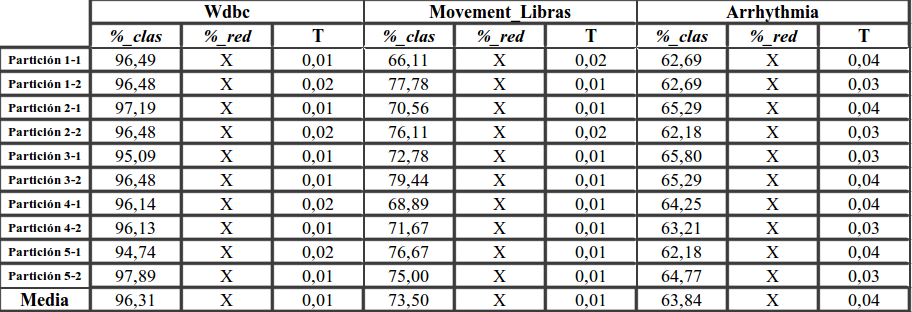
\includegraphics[width=1.0\linewidth]{3NN}
\caption{Experimentos para 3NN}
\label{fig:3NN}
\end{figure}

\begin{figure} [H]
\centering
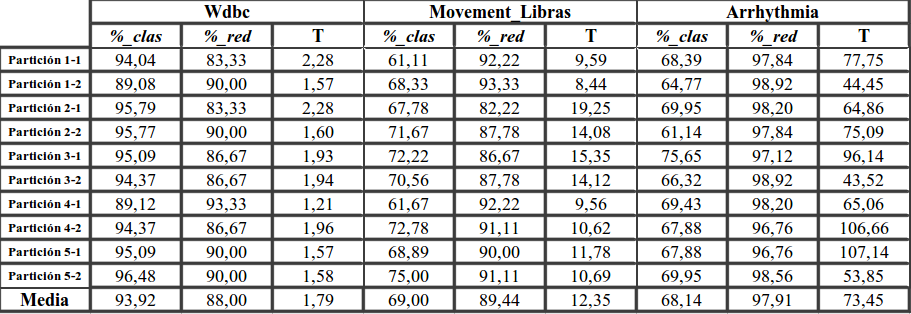
\includegraphics[width=1.0\linewidth]{SFS}
\caption{Experimentos para SFS (algoritmo de comparación)}
\label{fig:SFS}
\end{figure}

\begin{figure} [H]
\centering
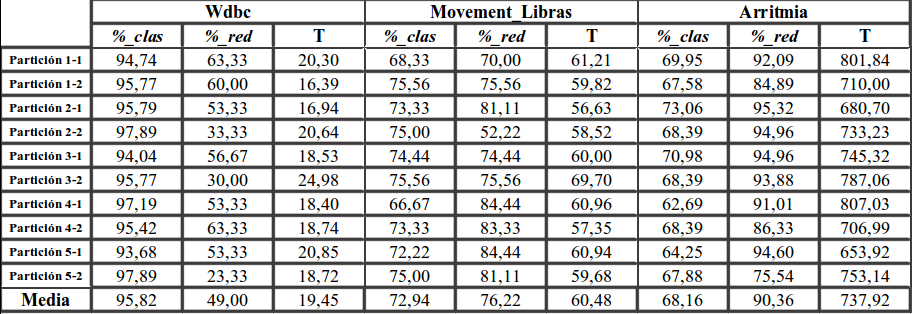
\includegraphics[width=1.0\linewidth]{BMB}
\caption{Experimentos para BMB}
\label{fig:BMB}
\end{figure}

\begin{figure} [H]
\centering
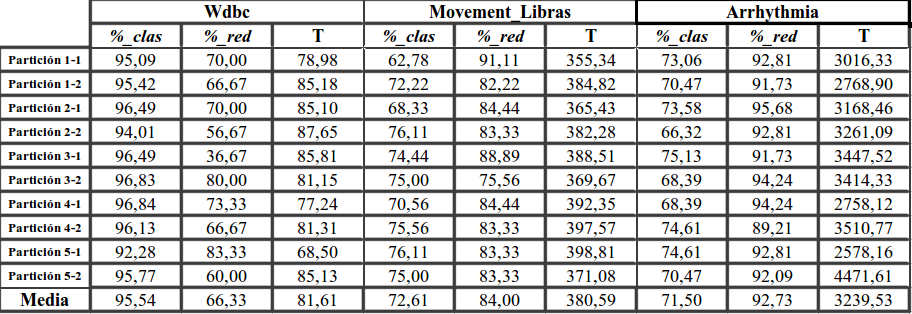
\includegraphics[width=1.0\linewidth]{GRASP}
\caption{Experimentos para GRASP}
\label{fig:GRASP}
\end{figure}

\begin{figure} [H]
\centering
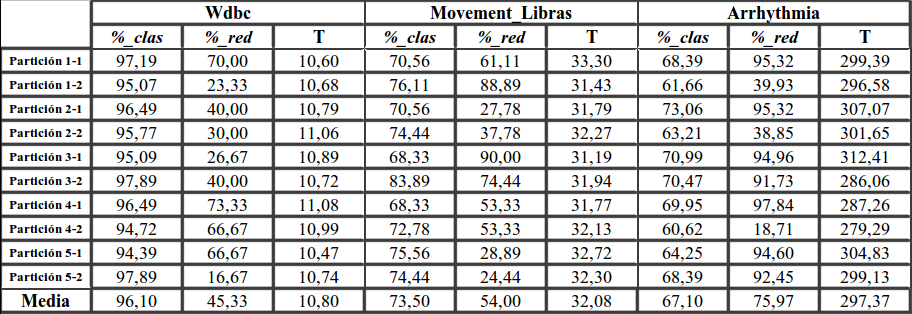
\includegraphics[width=1.0\linewidth]{ILS}
\caption{Experimentos para ILS}
\label{fig:ILS}
\end{figure}

\begin{figure} [H]
\centering
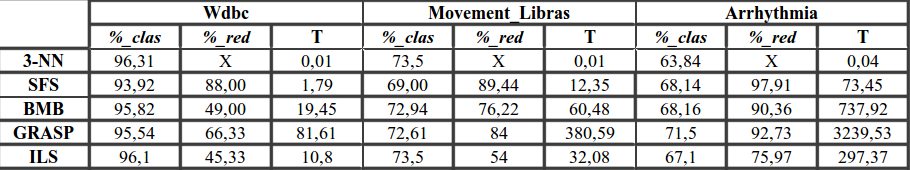
\includegraphics[width=1.0\linewidth]{TODOS}
\caption{Comparación de todos los algoritmos}
\label{fig:TODOS}
\end{figure}

Como podemos observar en esta última tabla, los resultados son muy parecidos para todos los algoritmos. 3-NN sin ninguna reducción en los vectores de características muestra mejor tasa de clase para WDBC y para movement libras por lo general. Esto se podría deber a que no hay mucho ruido entre las características, es decir, reduciendo las características siempre tenemos peores resultados porque quitamos datos importantes (y no ruidosos), o que no encontramos la solución óptima. En cambio, para la base de datos de Arrhythmia si vemos como obtenemos mejor tasa de clasificación tras aplicar los algoritmos de búsqueda que en el 3NN. Los datos de arrhythmia tienen un gran número de características, por lo que probablemente tengan más ruido que las otras 2 bases de datos.
\\
\\
En Arrhythmia también podemos ver que GRASP obtiene mucho mejores resultados que los demás algoritmos de búsqueda. Esto puede deberse a que en GRASP partimos de una solución muy buena (dada por el algoritmo greedy probabilístico) y lo que GRASP hace es aplicar búsqueda local sobre esta solución, es decir, queremos converger a una buena solución a partir de la ya dada por el greedy. En las demás bases de datos GRASP es levemente peor que los otros dos algoritmos. El hecho de que en Arrhythmia sea mejor y en las otras dos no, puede deberse al gran espacio de búsqueda que tiene esta base de datos. En las otras bases de datos, con espacios de búsqueda algo más pequeños, si puede darse que aplicando búsqueda local sobre una solución aleatoria termine dando su fruto.
\\
\\
En cuanto a ILS vemos como para WDBC da mejor resultado que BMB y GRASP. Esto se puede deber a que una vez encontramos una solución "medio buena" intensificamos sobre ésta aplicando mutaciones. Como vemos esto es mejor para espacios de búsqueda reducidos, ya que en estos casos puede resultar mejor aplicar una técnica de intensificación que de diversificación.
\\
\\
En cuanto a los tiempos vemos que el algoritmo más lento es GRASP. Esto es normal ya que para cada iteración tenemos que aplicar un algoritmo greedy que es costoso en tiempo. Este Greedy, además, es más costoso en tiempo que SFS, pues estamos introduciendo características de forma aleatoria y no siempre la mejor. Como vemos para la base de datos de Arrhythmia, llegamos a tiempos de hasta 4000 segundos, que es algo más de una hora por ejecución. BMB e ILS tienen tiempos algo más parecidos. Aún así, BMB es más lento y podría deberse a que BMB en cada iteración genera una nueva solución aleatoria, por lo que ya tiene que aplicar búsqueda local sobre una solución totalmente random y puede tardar en dejar de mejorar mucho tiempo. En cambio en ILS partimos de una solución aleatoria a la que le aplicamos la búsqueda local. Como recordamos, búsqueda local tenía como criterio de parada que dejara de mejorar, por lo tanto tras una ejecución de búsqueda local esa solución es más difícil que sea mejorable. Como en el resto de iteraciones la búsqueda local se aplica sobre pequeñas mutaciones de esa solución, es decir, a soluciones parecidas, entonces puede que por esta razón realice menos iteraciones (deje de mejorar antes).
\\
\\
A continuación dejo algunas gráficas ilustrativas de los resultados de los algoritmos para cada base de datos.

\begin{figure} [H]
\centering
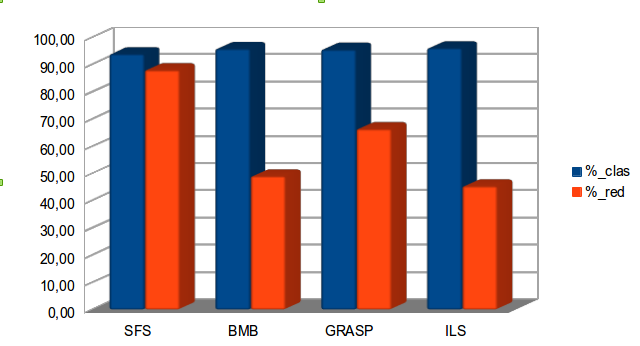
\includegraphics[width=1.0\linewidth]{GraficaWDBC}
\caption{Gráfico de resultados para la base de datos WDBC}
\label{fig:GraficaWDBC}
\end{figure}

\begin{figure} [H]
\centering
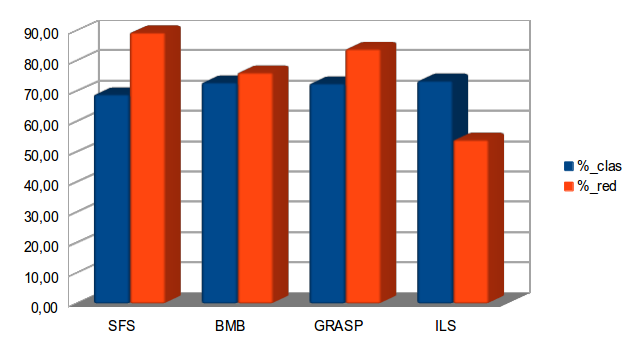
\includegraphics[width=1.0\linewidth]{graficaMovement}
\caption{Gráfico de resultados para la base de datos movement libras}
\label{fig:graficaMovement}
\end{figure}

\begin{figure} [H]
\centering
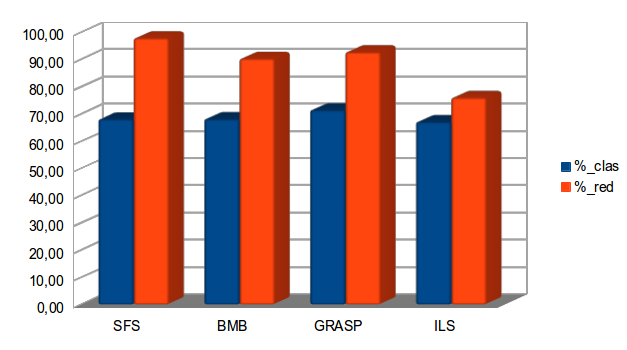
\includegraphics[width=1.0\linewidth]{Graficaarrhythmica}
\caption{Gráfico de resultados para la base de datos arrhythmia}
\label{fig:Graficaarrhythmica}
\end{figure}


\end{document}